\section{Preliminaries}
\label{section:prelim}

\par{
We frame spatial search using pictorial queries over a database of locations and their associated objects.
A \textit{pictorial query} is a canvas of points representing objects laid out in a spatial configuration of interest to the user.
\textit{Objects} and \textit{locations} are physical entities in the world, represented as points, with $(x,y)$ coordinates and names (often derived from geotag information).
We allow multiple objects of the same class or type, and assume objects have been assigned to their associated locations prior to search time.
For more detailed analysis of the motivation and methods for assigning objects to locations, see \textit{Geospatially Enhanced Search with Terrain Augmented Location Targeting (\textbf{GESTALT})}~\cite{Osul2023}.
Leveraging the data structures and algorithms that comprise \emph{COMPASS}, we apply one of three spatial search techniques to return a set of locations from the database that are associated with the object pattern of interest, as specified by the pictorial query. 
This search paradigm assumes that a user has knowledge of several objects and their spatial configuration, and wishes to retrieve a list of all locations that contain that same query configuration within a given \textit{region}, or area under search.
}

%suite of data structures and algorithms address the scalability for complex spatial pattern matching through representation, abstraction and pruning.
%In this section we introduce the terminology and intuition for our approaches, and briefly examine the enabling data structures. 
%We describe the algorithms in detail in section \ref{section:Methods} and provide a theoretical and empirical complexity analysis in section~\ref{section:results}.
%
%Our human-centric approach begins with our hierarchcal representation of space, which reflects how people tend to understand and remember the world. 
%Beginning from the largest elements, we divide the world into \textit{\textbf{regions}}, which could be a suburb, state or larger area depending on the use-case. 
%A region is the largest collection that we search over, and all of our algorithms assume the user has narrowed down to a region prior to searching with COMPASS.
%Rather than being defined explicilty by area, a region is a collection of \textit{\textbf{locations}}. 
%A location can be thought of as a place of some public significance or interest. 
%Locations contain \textit{\textbf{objects}} which are the things physically located in and around a location.
%At their core within COMPASS, objects consist of a \textit{\textbf{name}} which associates it with an object class and its \textit{\textbf{coordinates}}.

%Further detail on the data collection, assignment of objects to locations, and user interface are described in our introduction of the \textit{Geospatially Enhanced Search with Terrain Augmented Location Targeting (\textbf{GESTALT})} system \cite{osullivan2023}.


%In the event of ties, we apply the convention that the object that is more northern then western is dominant, and then we use lexicographic order.

\par{
To enable spatial search, \emph{COMPASS} abstracts the infinite spatial complexity of the world into one of two concise representations- a location-centric structure, or a concept map.
A \textit{location-centric structure} is a simple dictionary-based representation that describes a location by the objects contained in each of its 4 cardinal quadrants (Northwest, Northeast, Southwest, Southeast).
A \textit{concept map} can be used to represent a set of objects arranged spatially without explicitly encoding how they relate spatially to a location. \nrscomment{cite image concept map paper}
Entries in the matrix are either contain a $0$, representing empty space, or an object name, representing the position of that object.
Critically, concept maps are generated such that the relative order of objects from north to south and west to east is preserved from the original Cartesian representation, making them a condensed representation that captures the relevant spatial information needed to perform pattern matching.
Both location-centric structures and concept maps can be generated either from a pictorial query, or from a set of objects associated with a location. 
We implement concept maps using $N \times N$ matrices (where $N$ is the number of objects).
Figures~\ref{figure:ConceptMap-LO} and \ref{figure:conceptMap} show the abstraction process used to create and search over these two data structures.
}

%\par{
%COMPASS employs aggressive pruning strategies to reduce the complexity of multi-object spatial pattern matching to tractable levels. 
%The concept maps abstract away distance and absolute position, reducing the search complexity and also supporting the human-centric view of the world, where distance estimation is not required. 
%Finally, we build early-stopping into our search, meaning that as soon as a location is known to be a match, we return it and cease checking the remainder of that location.
%}
%A user who remembers three objects in a particular configuration is likely to be just as satisfied with the return of a location with boolean confidence as they are with a count of the number of times that configuration occurs, significantly reducing the number of possible configurations that must be explored to satisfy a query.
%Overall, COMPASS focuses on a search experience that supports the way a human interacts with and remembers the world, and made efforts to improve the tractability of that approach at each step, yielding a collection of data structures and algorithms that improve the human search experience.
%First is the implicit pruning of the search space by limiting the search area to regions.
%Next, while searching we employ the set-membership checks to exclude locations that cannot possibly satisfy the query, because they lack the objects required to fulfil it.
%An additional benefit of removing distance features is that it removes a map-centric criteria that people are typically very bad at estimating. 
%Another complexity reduction comes from focusing on maximizing recall by returning locations with any match. 
%The recall is checked by the logical step that as a person becomes more certain about a location they add more objects to the query, pruning the set of possible results dramatically with even just four or five query terms.


%\par{
%\emph{COMPASS} supports two forms of spatial relations: object-location relations and object-object relations.
%Both cases involve an offline encoding phase that enables an online search phase. 
%We discuss the details of the encoding phase in this section and leave the search details to section \ref{section:search}.
%}

\subsection{Object-Location relations}
Object-location relations encode cardinal directionality between objects and locations (i.e. whether an object is North, South, East, or West of a location). 
This type of information enables simple queries, such as when a user knows that a location has a lake on its western side. 
Each object-location relationship is defined independently of other objects associated with that location, and multiple constraints can be combined to form a more specific query, such as a lake west of the location and a pond south of the location.
Figure \ref{figure:ConceptMap-LO} shows how we encode a location (\ref{fig:CM-LO-Example}) as a geospatial index based on relative position to the location coordinates (\ref{fig:CM-LO-Setup}), and then how queries are processed (\ref{fig:CM-LO-Query}).
The search function returns the candidate locations ranked by the number of query terms that match the appropriate quadrant with respect to the location. \nrscomment{clean up this subsection}

\begin{figure*}[h]
    \centering
    \begin{subfigure}[t]{.25\textwidth}
        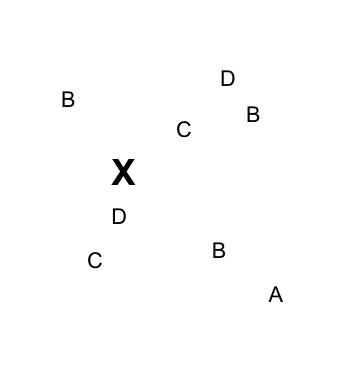
\includegraphics[width=\textwidth]{CM-ExampleLocation.png}
        \caption{\small A candidate location X has named objects A-D with the spatial layout depicted above.} 
        \label{fig:CM-LO-Example}
    \end{subfigure}
    \hfill
    \begin{subfigure}[t]{.25\textwidth}
        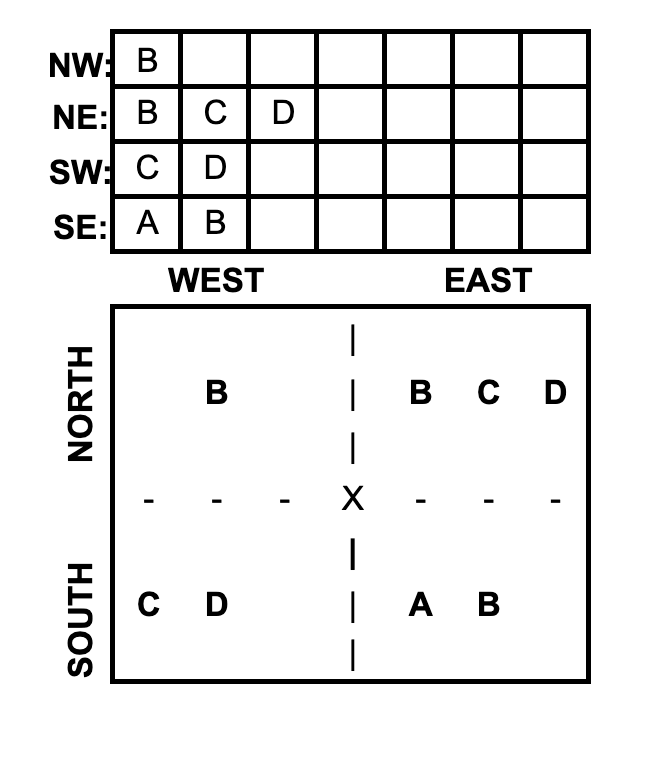
\includegraphics[width=\textwidth]{CM-LO-Setup.png}
        \caption{\small The objects are binned into spatial quadrants based on their relative position to the location coordinates, X.} 
        \label{fig:CM-LO-Setup}
    \end{subfigure}
    \hfill
        \begin{subfigure}[t]{.25\textwidth}
        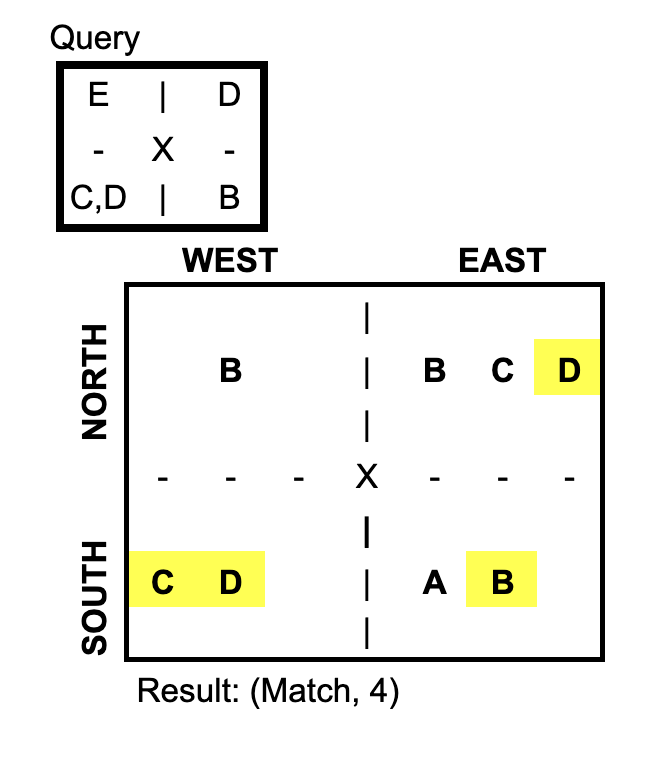
\includegraphics[width=\textwidth]{CM-LO-Query1.png}
        \caption{\small Rank the locations by the number of query terms that are found in the correct quadrant with respect to the location.}
        \label{fig:CM-LO-Query}
    \hfill
    \end{subfigure}
    \caption{\textbf{Object-Location Search Method. A Location-centric data structure (Figure \ref{fig:CM-LO-Setup}) is generated based on the cardinal relations between the objects and the location (Figure \ref{fig:CM-LO-Example}). Then a pictorial query is matched against the structure (Figure \ref{fig:CM-LO-Query}).}}\label{figure:ConceptMap-LO} 
\end{figure*}



\subsection{Object-Object relations}
The other type of spatial relationships we support searching are object-object relations, which are typically more complex than object-location relations.
Object-object relations refer to a configuration of objects that relate to one another spatially.
For example, a tree, a pond, and a sign might form a triangle, with each object having a directional constraint with respect to every other object in the query (i.e., tree upper left of pond, pond lower right of sign, and sign lower left of tree).
As the number of objects in the object-object configuration increases, the number of pairwise directional constraints needed to specify the query snowballs. 
%Object-object relations lend themselves particularly well to pictorial query specification~\cite{Soffer1997}.
%This method of specifying the spatial positioning of objects aligns nicely with how humans think about and describe landmarks in the world- by drawing a map. 
Figure \ref{figure:ConceptMap} shows how we encode a location (\ref{fig:CM-Example}) as a matrix of relative object positions (\ref{fig:CM-OO-Setup}) and then how queries are processed (\ref{fig:CM-OO-Query}).
The object-object approach to defining spatial configurations of objects is also more flexible than the object-location approach, which requires the user to know where each object lies in relation to the location. 

%In these circumstances, we can instead search for the relative position of objects to each other and ignore their absolute position within the location.


\begin{figure*}[h]
    \centering
    \begin{subfigure}[t]{.25\textwidth}
        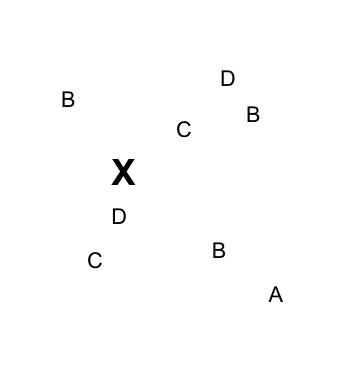
\includegraphics[width=\textwidth]{CM-ExampleLocation.png}
        \caption{\small A candidate location X has named objects A-D with the spatial layout depicted above.}
        \label{fig:CM-Example}
    \end{subfigure}
    \hfill
    \begin{subfigure}[t]{.25\textwidth}
        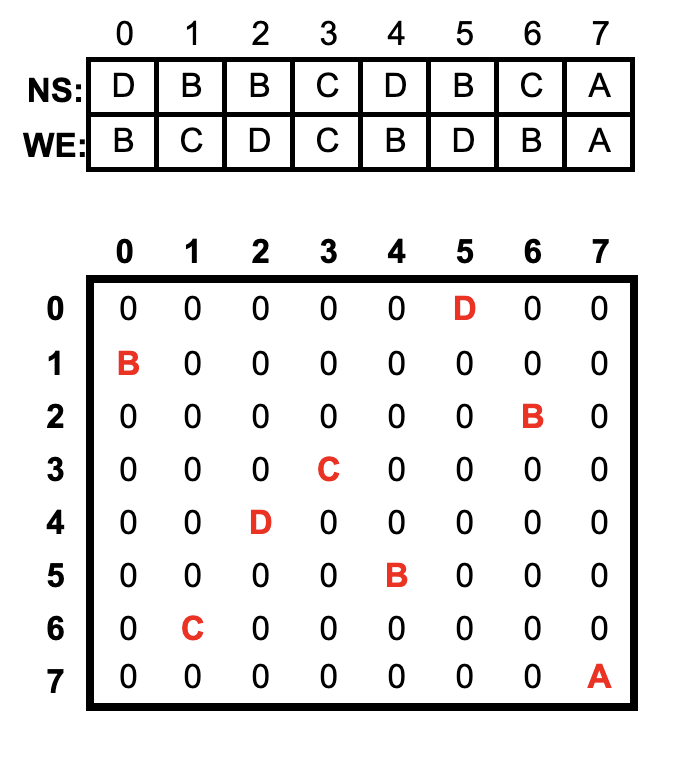
\includegraphics[width=\textwidth]{CM-OO-Setup.png}
        \caption{\small Objects associated with location X are ordered from North to South (NS) and West to East (WE) and mapped into a matrix with corresponding indices.}
        \label{fig:CM-OO-Setup}
    \end{subfigure}
    \hfill
        \begin{subfigure}[t]{.25\textwidth}
        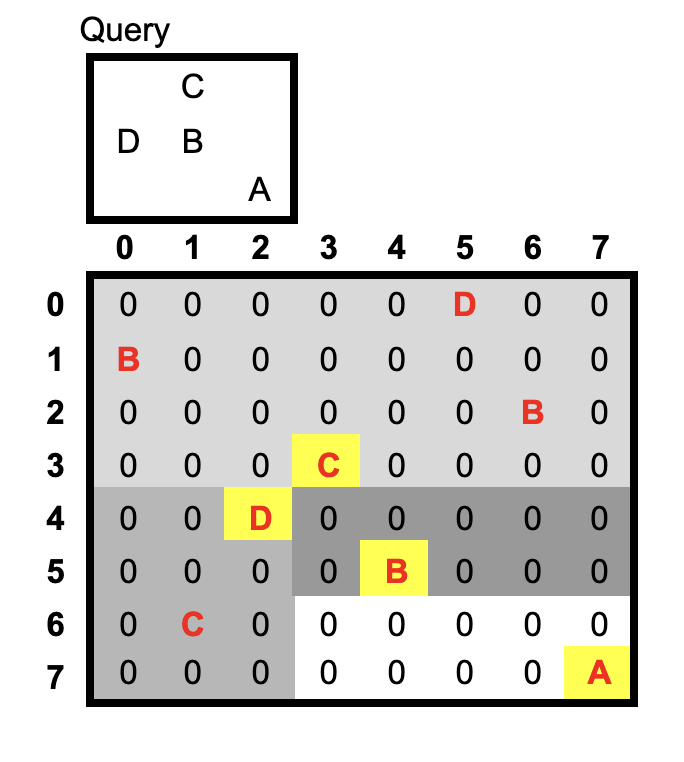
\includegraphics[width=\textwidth]{CM-OO-Query1.png}
        \caption{\small Recursive search. Each recursion is a darker shade, with an unpruned area in white. Objects highlighted in yellow are found to match the query configuration; candidate location X is a match for the query.}
        \label{fig:CM-OO-Query}
    \hfill
    \end{subfigure}
    \caption{\textbf{Object-Object Search Method. A Concept Map data structure (Figure \ref{fig:CM-OO-Setup}) is generated by ordering the objects associated with a candidate location (Figure \ref{fig:CM-Example}) from North to South and West to East. The search step (Figure \ref{fig:CM-OO-Query}) then recursively prunes the concept map until ANY matching configuration of objects is identified, or the query constraints are found not to be satisfied.
    }}\label{figure:ConceptMap} 
\end{figure*}

%\subsection{Cardinality Invariant Object-Object relations}
%Cardinality Invariant Object-Object relations refer to a variant of object-object spatial relations such that 
%\nrscomment{describe here}
%\nrscomment{diagram here}










%To encode a location, we begin by setting the centroid of the location provided by OSM during Data Acquisition to be the root of a quartering of the search space into NorthWest, NorthEast, SouthWest and SouthEast quadrants. 
%Each object's coordinates are compared to the location centroid and it is assigned to the appropriate quadrant. 
%Where a point lies on the border we adopt the convention that it belongs to the southern and western quadrants. 
%To query the location-object index, a user imagines themselves standing at the centre of the location and enters the query terms into the quadrant they believe it belongs in. 
%That query map is then compared to each candidate location. An object in the query is in the same quadrant as an object in a candidate location, the number of correct terms increments.
%The result is a matrix in which each row and column has only a single object. 
%Where ties are experienced in the real world (due to a lack of GPS precision, or very close position) they are broken lexicographically in the object-object concept map instantiation.
%To generate the object-object matrix concept map, we sort all objects from north to south in one list, and all objects west to east in another. Their position in the matrix is then determined by their position in the matrix. For example in figure ref{{fig:CM-OO-Setup}} object \textbf{"A"} is in the 8th position from the North, and the 8th Position from the west, so in the matrix it is assigned to index [0,0].
%To then query this sparse matrix, approached it as you might approach looking for something on a map - by eliminating confusing or redundant information until we are left with a very simple question to answer. 
%We would probably just zoom in a little closer on our mapping software to see if we can see the arrangement of objects we are looking for - and so our approach mimics the 'zooming-in' approach.
%Our implemenation aggressively prunes the search space using recursive grid search \osullikomment{Cite}. In Figure \ref{CM-OO-Query} the query has a "C" object as the most northern object. 
%So, we can prune the entire search space north of the north most C, because no matches in that region can satisfy the query. 
%Next, recurse and we prune on the matrix from the west, knowing that no terms west of the west-most D can possibly satisfy the query. 
%The pruning continues from the north, then the south until there is only a single search term left. 
%If that term exists anywhere in the unpruned area, the query matches. 
%Note that this approach returns any collection of objects that match the pattern specified in the query, regardless of other objects being present or how many times the sub-pattern occurs in the query space. 


%The process of creating and querying a concept map is shown in Figure \ref{figure:ConceptMap}.



% This all belongs in search
%\subsubsection{Query Input}
%- algorithm for parsing from grid, etc.
%\subsubsection{Solution}
%- recursive algorithm for finding any match
%- complexity analysis
%
%\subsubsection{Experimental Results?}
%- on ground truth queries? report number of locations pruned? timings?

%Concept mapping has been partially implemented in Python leveraging the \textit{Scipy} library\footnote{\href{https://pypi.org/project/scipy/}{SciPy PyPI Repo}}. Two different approaches have been trialed. 
%The first is simple dynamic arithmetic on the coordinates stored in a Pandas data frame. If one set of coordinates is above, below, left or right of another, it is north, south, east or west, respectively. 
%While these calculations are in constant time for straightforward comparisons of known objects (e.g. "is the pond west of the bridge"), the time complexity rapidly increases as soon as aggregations are employed. 
%Queries of "Give me everything west of the duck pond" would execute in $O(N)$ time as each element has to be examined. Worst-case queries would run in $O(N\sup{2})$ time, where every object is checked for its position relative to every other object. 

%The second (better) approach (only partially implemented) instantiates the objects within a location into a KD-Tree. 
%Assuming that the object centroid is the root, we can quickly complete queries like "Give me everything west of the duck pond" by leveraging the structure of the subtrees to return the requested set. 
%Similarly, getting the relative positions of two objects searches for a common ancestor. It uses the path between the children and their ancestor node to infer their spatial relation to each other.

%A third approach, designed to leverage the \textit{Neo4J Python Library}\footnote{\href{https://pypi.org/project/neo4j/}{Neo4J PyPI Repo}} to connect to a \textit{Neo4J Graph Database}\footnote{\href{https://neo4j.com/}{Neo4J Website}} but not implemented frames concept mapping as a graph traversal problem. 
%In this formulation, each object is a node on a graph. Weighted, labeled edges exist between each node within a given proximity threshold to the node. 
%The edge labels describe the neighboring node's cardinal direction and the distance weights. 
%After constructing the object graph, queries for 'give me everything west of the duck pond' would freely explore nodes connected by west, north and south edges. 
%It can only traverse along an east edge so long as the total cost of traveling east would be less than the cumulative value of the 'west' travel up to this point. 

%%Overall, concept mapping aims to enable geographic search over objects by explicitly representing their geospatial relationships to each other. 
%The author implemented a very basic approach using coordinate arithmetic was quickly determined to be infeasible for the extensive data sets that \textit{GESTALT} anticipates processing. 
%KD-Trees for the objects in each location have been implemented, as have the KD-Trees for the locations themselves. 
%This conceptual KD-Tree of KD-Trees approach performs a natural aggregation function which, provided that regions are created consistently, will allow for relative spatial queries at different levels of granularity. 
%Empirical evaluation of the performance of the arithmetic, KD-Tree and Graph-based approaches is yet to be completed. 


%%%%%%%%%%%%%%%NSCH clean up, incorporate, and delete the text below this point
%The first is \textit{Static Cardinal Relations} which encodes whether an object is North, South, East or West of a location. Static Cardinal Relations support simple queries where the user knows that a location has a lake on its western side. 
%The second is \textit{Dynamic Cardinal Relations} which determines whether an object is North, South, East or West of another object within a location. These queries support cases where a searcher might remember standing at a lake northeast of a location and that there was a swingset to the immediate west of them but still in the northeast of the location overall. 


%Concept mapping needs to be unsupervised and support aggregation. Tracking every object's relative location to every other object quickly becomes intractable, so mechanisms to aggregate depending on the level of granularity need to be applied. 
%Accordingly, the underlying data structure must support aggregation and relative position querying. 